% arxiv-twocolumn.latex: the shared pandoc template for a two-column arXiv-style preprint.
% Built by build_paper.py (pandoc, then tectonic or any XeLaTeX); arxiv-twocolumn.lua is its filter.
% Engine: XeTeX (fontspec, unicode-math). Fonts: Latin Modern text and math, DejaVu Sans Mono for code;
% a character the current font lacks falls back to Latin Modern Math, then to DejaVu Sans.
\documentclass[10pt,letterpaper,twocolumn]{article}
\usepackage[letterpaper,top=0.75in,bottom=0.9in,left=0.7in,right=0.7in,columnsep=0.25in]{geometry}
\usepackage{amsmath}
\usepackage{fontspec}
\usepackage{unicode-math}
\setmainfont{lmroman10}[Extension=.otf,UprightFont=*-regular,BoldFont=*-bold,ItalicFont=*-italic,BoldItalicFont=*-bolditalic]
\setsansfont{lmsans10}[Extension=.otf,UprightFont=*-regular,BoldFont=*-bold,ItalicFont=*-oblique,BoldItalicFont=*-boldoblique]
\setmonofont{DejaVuSansMono}[Extension=.ttf,UprightFont=*,BoldFont=*-Bold,ItalicFont=*-Oblique,BoldItalicFont=*-BoldOblique,Scale=MatchLowercase]
\setmathfont{latinmodern-math.otf}
\newfontfamily\typesetfallbackmath{latinmodern-math.otf}
\newfontfamily\typesetfallbacksans{DejaVuSans}[Extension=.ttf,UprightFont=*,BoldFont=*-Bold,ItalicFont=*-Oblique,BoldItalicFont=*-BoldOblique]
% \typesetmap{"XXXX} (build_paper.py writes one for each character outside Latin-1 and Latin
% Extended-A that the paper uses) makes the character active at the start of the document: in text it
% comes from the current font when that has it, else from the first fallback that does; in math it
% keeps whatever unicode-math gave it (a prime stays a prime).
\makeatletter
\protected\def\typesetglyph#1{%
  \iffontchar\font#1\relax\char#1\relax
  \else{\typesetfallbackmath\iffontchar\font#1\relax\char#1\relax\else\typesetfallbacksans\char#1\relax\fi}%
  \fi}
\def\typeset@math#1{%
  \ifcsname typeset@m@#1\endcsname\csname typeset@m@#1\expandafter\endcsname\else\Uchar#1 \fi}
\protected\def\typesetchar#1{\ifmmode\expandafter\typeset@math\else\expandafter\typesetglyph\fi{#1}}
\def\typesetmap#1{%
  \edef\typeset@n{\number#1}% outside \lowercase, which would lowercase the hex digits A-F
  \begingroup\lccode`\~=\typeset@n\relax
  \lowercase{\endgroup
    \ifdefined~\expandafter\let\csname typeset@m@\typeset@n\endcsname~\fi
    \edef~{\noexpand\typesetchar{\typeset@n}}}%
  \catcode\typeset@n=13\relax}
\makeatother
% amssymb names that unicode-math spells differently.
\AtBeginDocument{%
  \providecommand{\square}{\mdlgwhtsquare}\providecommand{\Box}{\mdlgwhtsquare}%
  \providecommand{\blacksquare}{\mdlgblksquare}\providecommand{\lozenge}{\mdlgwhtlozenge}%
  \providecommand{\blacklozenge}{\mdlgblklozenge}}
% Legacy two-letter font commands (\rm, \bf, \it, ...), in text and in math.
\providecommand{\rm}{}\DeclareOldFontCommand{\rm}{\normalfont\rmfamily}{\mathrm}
\providecommand{\bf}{}\DeclareOldFontCommand{\bf}{\normalfont\bfseries}{\mathbf}
\providecommand{\it}{}\DeclareOldFontCommand{\it}{\normalfont\itshape}{\mathit}
\providecommand{\sf}{}\DeclareOldFontCommand{\sf}{\normalfont\sffamily}{\mathsf}
\providecommand{\tt}{}\DeclareOldFontCommand{\tt}{\normalfont\ttfamily}{\mathtt}
\usepackage{microtype}
\usepackage[dvipsnames]{xcolor}
\usepackage{graphicx}
\usepackage{booktabs}
\usepackage{array}
\usepackage{ragged2e}
\usepackage{xtab}
\usepackage{cuted}
\usepackage{caption}
\captionsetup{font=small,labelfont=bf,skip=4pt}
\captionsetup[table]{position=top}
\usepackage{fvextra}
\usepackage{xurl}
\usepackage{titlesec}
\usepackage{fancyhdr}
\usepackage{footmisc}
\usepackage{enumitem}
\setlist{itemsep=1pt,topsep=3pt,parsep=0pt}
\usepackage{hyperref}
\hypersetup{colorlinks=true,linkcolor=MidnightBlue,citecolor=MidnightBlue,urlcolor=MidnightBlue,filecolor=MidnightBlue,
  pdftitle={An untuned rank-selection and reconstruction procedure recovers CHIME/FRB burst morphology},pdfauthor={Ikailo John Sessford},pdfcreator={pandoc + XeTeX},bookmarksnumbered=true}
\pdfstringdefDisableCommands{\def\typesetchar#1{\Uchar#1 }}

% Paragraphs: indented, no extra space, ragged bottom so columns do not stretch.
\setlength{\parskip}{0pt}
\raggedbottom
\emergencystretch=1.5em
\tolerance=1000
\hbadness=10000
\clubpenalty=10000
\widowpenalty=10000

% Section headings. Numbered only when the paper's own headings carry no numbers (build_paper.py decides).
\setcounter{secnumdepth}{-\maxdimen}
\titleformat*{\section}{\normalfont\large\bfseries\raggedright}
\titleformat*{\subsection}{\normalfont\normalsize\bfseries\raggedright}
\titleformat*{\subsubsection}{\normalfont\normalsize\bfseries\itshape\raggedright}
\titleformat*{\paragraph}{\normalfont\normalsize\itshape}
\titlespacing*{\section}{0pt}{2.0ex plus 1ex minus .2ex}{1.0ex plus .2ex}
\titlespacing*{\subsection}{0pt}{1.6ex plus 1ex minus .2ex}{0.6ex plus .2ex}
\titlespacing*{\subsubsection}{0pt}{1.4ex plus 1ex minus .2ex}{0.5ex plus .2ex}
\titlespacing*{\paragraph}{0pt}{1.0ex plus .5ex}{0.6em}

% Code: monospaced at the floor size, wrapped at the column edge and never scaled.
\RecustomVerbatimEnvironment{verbatim}{Verbatim}{fontsize=\footnotesize,breaklines=true,breakanywhere=true,breaksymbolleft={},
  xleftmargin=0.5em,frame=leftline,framerule=0.4pt,rulecolor=\color{Gray},framesep=0.5em}

% Tables: small type, tight columns. Long tables break across columns (xtabular); wide ones float full width.
\setlength{\tabcolsep}{4pt}
\renewcommand{\arraystretch}{1.1}
\newcolumntype{L}[1]{>{\RaggedRight\arraybackslash}p{#1}}
\newcolumntype{R}[1]{>{\RaggedLeft\arraybackslash}p{#1}}
\newcolumntype{C}[1]{>{\Centering\arraybackslash}p{#1}}
% Scaling has a floor: nothing is set smaller than \typesetfloor.
% DERIVED: 8 pt is \footnotesize of this 10 pt class, the smallest running text the template sets
% (tables, code), so a scaled display is never smaller than the smallest text already on the page.
\newdimen\typesetfloor \typesetfloor=8pt
\newsavebox{\typesetfitbox}
\newif\iftypesetfitok
\makeatletter
% \typeset@try{width}{base size}: does \typesetfitbox fit in width, scaled no smaller than the floor?
% Sets \iftypesetfitok, and logs the scale it would apply ("typeset-scale: <scale x 1000>").
\def\typeset@try#1#2{%
  \ifdim\wd\typesetfitbox>#1\relax
    \edef\typeset@scale{\the\numexpr\number\dimexpr#1\relax*1000/\number\wd\typesetfitbox\relax}%
    % the effective size, base size x scale, against the floor
    \ifdim\dimexpr#2*\typeset@scale/1000\relax<\typesetfloor
      \typesetfitokfalse
    \else
      \typesetfitoktrue\typeout{typeset-scale: \typeset@scale}%
    \fi
  \else
    \typesetfitoktrue
  \fi}
% \typesetfit{width}{content}: the content at natural size, scaled down only when wider than width,
% and never below the floor; content too wide even at the floor is set at the floor and overflows,
% which the build reports ("typeset-overflow").
\newcommand{\typesetfit}[2]{\sbox{\typesetfitbox}{#2}\typeset@place{#1}{\f@size pt}}
\def\typeset@place#1#2{%
  \typeset@try{#1}{#2}%
  \iftypesetfitok
    \ifdim\wd\typesetfitbox>#1\relax\resizebox{#1}{!}{\usebox{\typesetfitbox}}\else\usebox{\typesetfitbox}\fi
  \else
    \edef\typeset@floorscale{\the\numexpr\number\typesetfloor*1000/\number\dimexpr#2\relax\relax}%
    \ifnum\typeset@floorscale<1000
      \typeout{typeset-scale: \typeset@floorscale}%
      \scalebox{\strip@pt\dimexpr\typeset@floorscale pt/1000\relax}{\usebox{\typesetfitbox}}%
    \else
      \usebox{\typesetfitbox}%
    \fi
    \typeout{typeset-overflow: \the\wd\typesetfitbox\space into \the\dimexpr#1\relax}%
  \fi}
% \typesetdisplay{math}{split}: a display equation, and the same equation broken into lines at its
% top-level \qquad separators (empty when it has none). The first of these that fits, never below the
% floor, is used: the equation in the column; the split form in the column; the equation across both
% columns (a strip at this point of the text); the split form across both columns.
\def\typeset@show{%
  \[\ifdim\wd\typesetfitbox>\linewidth\resizebox{\linewidth}{!}{\usebox{\typesetfitbox}}\else\usebox{\typesetfitbox}\fi\]}
\def\typeset@strip{%
  \typeout{typeset-strip: display}%
  \par\begin{strip}\vspace{-\abovedisplayskip}\[\typeset@place{\textwidth}{\f@size pt}\]\vspace{-\belowdisplayskip}\end{strip}%
  \noindent\ignorespaces}
\long\def\typesetdisplay#1#2{%
  \sbox{\typesetfitbox}{\(\displaystyle #1\)}%
  \typeset@try{\linewidth}{\f@size pt}%
  \iftypesetfitok\typeset@show\else
    \long\def\typeset@alt{#2}%
    \ifx\typeset@alt\@empty\typeset@strip\else
      \sbox{\typesetfitbox}{\(\displaystyle #2\)}%
      \typeset@try{\linewidth}{\f@size pt}%
      \iftypesetfitok\typeset@show\else
        \sbox{\typesetfitbox}{\(\displaystyle #1\)}%
        \typeset@try{\textwidth}{\f@size pt}%
        \iftypesetfitok\else\sbox{\typesetfitbox}{\(\displaystyle #2\)}\fi
        \typeset@strip
      \fi
    \fi
  \fi}
% \typesetcolumntable{tabular}: an in-column table at natural size, in the column if it fits there
% (tables are already at the floor size, so they are never scaled), otherwise across both columns.
\long\def\typesetcolumntable#1{%
  \sbox{\typesetfitbox}{\footnotesize #1}%
  \ifdim\wd\typesetfitbox>\linewidth
    \typeout{typeset-strip: table}%
    \begin{strip}\centering\typeset@place{\textwidth}{\typesetfloor}\par\end{strip}%
  \else
    \begin{center}\usebox{\typesetfitbox}\end{center}%
  \fi}
\makeatother

% For the build's report: how full each column is when it is made ("typeset-column: page columns
% text floats height", lengths in sp). Float-only pages are made elsewhere and are not logged.
\usepackage{etoolbox}
\makeatletter
\def\typeset@colfill{%
  \setbox\z@\vbox{\unvcopy\@cclv}%
  \typeout{typeset-column: \number\c@page\space\if@twocolumn 2\else 1\fi\space
    \number\dimexpr\ht\z@+\dp\z@+\ht\footins+\dp\footins\relax\space
    \number\dimexpr\textheight-\@colroom\relax\space\number\textheight}}
\pretocmd{\@makecol}{\typeset@colfill}{}{\typeout{typeset-column: unavailable}}
% A heading above the paper's section level (a part of the paper) is set as a centred divider.
\newcounter{typesetpart}
\newcommand{\typesetpart}[2]{\par\vspace{2.5ex plus 1ex}\stepcounter{typesetpart}%
  \pdfbookmark[0]{#2}{typesetpart.\arabic{typesetpart}}%
  {\centering\large\bfseries #1\par}\vspace{1.5ex plus .5ex}}
\makeatother

% Floats: allow full-width floats to take most of a page, and many to queue.
\renewcommand{\topfraction}{0.9}
\renewcommand{\bottomfraction}{0.8}
\renewcommand{\textfraction}{0.07}
\renewcommand{\floatpagefraction}{0.75}
\renewcommand{\dbltopfraction}{0.9}
\renewcommand{\dblfloatpagefraction}{0.75}
\setcounter{topnumber}{3}
\setcounter{dbltopnumber}{3}
\setcounter{totalnumber}{5}
\extrafloats{200}
\setkeys{Gin}{width=\linewidth,height=0.8\textheight,keepaspectratio}

% Pandoc helpers.
\providecommand{\tightlist}{\setlength{\itemsep}{0pt}\setlength{\parskip}{0pt}}
\providecommand{\pandocbounded}[1]{#1}
\newcommand{\passthrough}[1]{#1}

\pagestyle{fancy}
\fancyhf{}
\renewcommand{\headrulewidth}{0pt}
\fancyfoot[C]{\small\thepage}
\fancypagestyle{plain}{\fancyhf{}\renewcommand{\headrulewidth}{0pt}\fancyfoot[C]{\small\thepage}}

\AtBeginDocument{%
\typesetmap{"2212}% −
}

\begin{document}

% Title block across both columns, with the abstract under it when the two leave room for the body to
% start on page 1; otherwise the abstract opens the two-column body, so no page is left near-empty.
\makeatletter
\newsavebox{\typesettitle}
\newsavebox{\typesetfront}
\setbox\typesettitle=\vbox{%
  \hsize=\textwidth \linewidth=\textwidth \columnwidth=\textwidth
  \begingroup\centering
  {\LARGE\bfseries An untuned rank-selection and reconstruction procedure recovers CHIME/FRB burst morphology\par}
  \vspace{0.8ex}{\large Applied to public Catalog 1 waterfalls, with no per-substrate tuning and no burst template.\par}
  \vspace{1.8ex}
  {\normalsize Ikailo John Sessford\par}
  \vspace{0.3ex}
  {\small\itshape Ikailo Inc.\par}
  {\small \href{mailto:john@ikailo.com}{\texttt{john@ikailo.com}}\quad ORCID \href{https://orcid.org/0009-0002-0150-4027}{0009-0002-0150-4027}\par}
  \vspace{0.6ex}{\small Pre-print. November 2026.\par}
  \endgroup
}
\long\def\typesetrule{\vspace{1.6ex}\noindent\rule{\linewidth}{0.4pt}\par\vspace{1.5ex}}
\long\def\typesetabstract{%
We apply a parameter-free rank-selection and reconstruction procedure to publicly released CHIME/FRB Catalog 1 waterfalls and compare the result against CHIME's own \emph{fitburst} forward model. The procedure selects its rank against a noise floor derived from the Tracy--Widom law of a pure-noise screen, reconstructs the field as the orthogonal projection onto its resolved modes --- lossless, with everything else kept in a residual --- and moves persistent narrowband structure to that residual by a geometric cut on each mode's entropic footprint. No constant is fitted to the data, no template of a burst enters anywhere, and nothing is tuned per event. On four bright events the reconstruction correlates with the forward model at \(0.421\)--\(0.533\) (mean \(0.470\)), against \(0.115\)--\(0.373\) (mean \(0.198\)) for the raw waterfall and \(0.214\) for a box-average control that applies frequency smoothing alone. To make those figures interpretable in the absence of ground truth we report two reference points: the forward model corrupted by the record's own measured noise scores \(0.219\) against the model, and the forward model degraded by exactly the resolution the modes are read at scores \(0.994\). The read therefore sits well above what the record's noise permits and well below what that resolution permits. It is taken at the recorded channel resolution and keeps structure along frequency that the smooth forward model does not carry; the remaining gap reflects that structure and the forward model's own parametric form, which we cannot separate without refitting the model. A further 12 waterfalls drawn uniformly at random from the same release are read by the identical path; all twelve are read without incident and eight resolve a mode above the floor. Neither the read nor the forward model is ground truth, and the noise floor is calibrated against an i.i.d. bulk which a serially correlated record violates; both limits are stated and quantified.
}
\setbox\typesetfront=\vbox{%
  \hsize=\textwidth \linewidth=\textwidth \columnwidth=\textwidth
  \unvcopy\typesettitle
  \vspace{2ex}
  {\centering\small\bfseries Abstract\par}
  \vspace{0.6ex}
  \begin{list}{}{\setlength{\leftmargin}{0.06\textwidth}\setlength{\rightmargin}{0.06\textwidth}%
    \setlength{\listparindent}{1.2em}\setlength{\itemindent}{0pt}\setlength{\parsep}{0.5ex}\setlength{\topsep}{0pt}}
  \small\item\relax\typesetabstract
  \end{list}
  \typesetrule
}
% CHOSEN: the title block and abstract go across both columns only if they leave ten lines of each
% column for the body on page 1. Ten lines is about a sixth of the page: enough that page 1 reads as
% the start of the paper, small enough that only a long abstract moves into the columns.
\ifdim\dimexpr\ht\typesetfront+\dp\typesetfront+10\baselineskip\relax<\textheight
  \twocolumn[\unvbox\typesetfront]
\else
  \twocolumn[\unvbox\typesettitle\typesetrule]
  {\centering\small\bfseries Abstract\par}\vspace{0.6ex}
  {\small\setlength{\parskip}{0.5ex}\noindent\typesetabstract\par}
  \typesetrule
\fi
\makeatother

\section{1. Introduction}\label{1-introduction}

A dedispersed fast radio burst waterfall is a two-dimensional array of intensity against frequency and time, carrying a burst of unknown morphology on a noise background, with a substantial fraction of its channels lost to radio-frequency interference (RFI) or to instrumental masking. Two questions have to be answered before anything can be said about the burst: how many degrees of freedom in the record are signal rather than noise, and which parts of the measured field to keep.

Both are usually answered with a model. A forward model fixes the burst's functional form --- CHIME's \emph{fitburst} uses Gaussians in time against a running power law in frequency --- and solves for that form's parameters; RFI excision applies thresholds tuned per instrument and often per observation. Both approaches work, and both make the answer depend on choices the analyst supplies.

This paper reports what happens when neither is supplied. We apply the read-side filter of the \emph{entroptics} construction {[}Sessford 2026{]} to public CHIME/FRB Catalog 1 waterfalls and compare its output against \emph{fitburst} on the same records.

\textbf{What ``untuned'' means here.} It is a specific and checkable claim, not a rhetorical one:

\begin{enumerate}
\def\labelenumi{\arabic{enumi}.}
\tightlist
\item
  \textbf{No constant is fitted to data or calibrated to a substrate.} Every fixed number in the procedure is a derived mathematical quantity --- a \(\chi^2\) median {[}Wilson \& Hilferty 1931{]}, an influence-function variance, a universal Tracy--Widom quantile --- or a stated criterion. The provenance of each is tabulated in the instrument paper {[}Sessford 2026, §11.1{]}.
\item
  \textbf{Nothing is set per event.} The same call is made on all sixteen waterfalls read here, with the same arguments. Nothing is inspected and adjusted between events.
\item
  \textbf{No template of a burst enters.} The reconstruction is supported on the measured screen's own singular vectors and synthesises nothing.
\item
  \textbf{What the reader does supply} is an operating point: a false-alarm level \(\alpha\), which by the Neyman--Pearson lemma encodes the relative cost of a false alarm against a miss and cannot be derived from the data, together with the null it is taken against. Both are left at their defaults throughout (\(\alpha=0.05\), the derived edge). Two facts about the record are declared rather than inferred: which axis is ordered, and that the feature channels are commensurate.
\end{enumerate}

The claim under test is transfer, not accuracy. The construction is validated on synthetic signals with a planted ground truth {[}Sessford 2026, §12{]}; a real substrate tests whether the same untuned instrument still works when nobody chose the record.

\section{2. Method}\label{2-method}

This section is self-contained enough to follow without the instrument paper, which carries the definitions, the proofs and the provenance of every constant {[}Sessford 2026{]}.

Write \(W\in\mathbb{R}^{T\times F}\) for the dedispersed waterfall with \(T\) time samples and \(F\) frequency channels, the time axis \emph{ordered} and the frequency axis carrying commensurate channels.

\textbf{Observer facts.} Dead channels are \emph{dropped}, never zero-filled. A channel that was measured and read zero is an observation of no power; a channel that was never measured is absent, and absence is not an observation of zero --- substituting zero widens the axis the signal is scored against by exactly the channels carrying nothing. ``Dead'' is the catalogue's own mask together with a zero-variance test. This is the only step that uses knowledge of the instrument, and it supplies no burst information.

\textbf{Whiten.} Each surviving channel is centred on its mean and scaled by its root-mean-square deviation about it, so every whitened channel carries the same energy and the screen's Gram is a sample correlation matrix. A channel whose values are all equal has no scale and leaves the screen; no number separates it from one that moved. The step equalises per-channel scale and performs no decorrelation --- it is a per-channel divide, not \(\Sigma^{-1/2}\) --- so noise correlated \emph{across} channels survives it intact.

\textbf{Fold.} The frequency axis is coarsened to the resolution the record's own power marginal says it carries, \(F_{\mathrm{eff}}=\operatorname{round}(F/\delta_F)\) with \(\delta_F=F_{\mathrm{eff}\text{-}\mathrm{measured}}/2^{\mathrm H_F}\) read from the Shannon entropy of the frequency power marginal. The fold is licensed only where two conditions both hold: that the concentration is real against an exact Dirichlet null, and that the frequency axis is \emph{continuous} --- that neighbouring channels are more alike than a random relabelling, tested against the closed-form permutation null. The time axis keeps native spacing, which the ordered reads require. For these frames the fold takes \(9{,}760\)--\(11{,}696\) live channels to \(5{,}949\)--\(10{,}972\).

\textbf{The derived floor.} The largest squared singular value of an \(N\times F_{\mathrm{eff}}\) pure-noise screen concentrates at the Johnstone centre \(\mu=(\sqrt{N-1}+\sqrt{F_{\mathrm{eff}}})^2\) with fluctuation scale \(\varsigma_J=(\sqrt{N-1}+\sqrt{F_{\mathrm{eff}}})\big(\tfrac1{\sqrt{N-1}}+\tfrac1{\sqrt{F_{\mathrm{eff}}}}\big)^{1/3}\), and \((s_1^2-\mu)/\varsigma_J\) follows the real (\(\beta=1\)) Tracy--Widom law {[}Tracy \& Widom 1996; Johnstone 2001{]}. The per-cell variance is the screen's mean cell energy with the centring's degree of freedom, \(\hat\sigma^2=\|S\|_F^2/(N F_{\mathrm{eff}})\cdot N/(N-1)\). Every whitened channel has the same energy, so on an unfolded screen this is the null's own variance exactly; these screens are folded, where channels that share structure raise it, which only raises the floor. The edge law is proved for i.i.d. entries with a finite fourth moment {[}Bao, Pan \& Zhou 2012{]}. With the universal Tracy--Widom\(_1\) quantile \(q_\alpha\) (\(q_{0.05}=0.9793\)),

\typesetdisplay{\Phi=\sqrt{\hat\sigma^2\,(\mu+q_\alpha\varsigma_J)},\qquad K_{\mathrm{signal}}=\#\{k:s_k>\Phi\}.}{\begin{gathered}\Phi=\sqrt{\hat\sigma^2\,(\mu+q_\alpha\varsigma_J)},\\ K_{\mathrm{signal}}=\#\{k:s_k>\Phi\}.\end{gathered}}

Given \(\alpha\), \(\mu,\varsigma_J\) and \((N-1)/N\) depend on the shape \((N,F_{\mathrm{eff}})\) alone and \(q_\alpha\) is a universal constant. Nothing in \(\Phi\) is fitted.

\textbf{The mode footprint.} Each resolved mode carries a left (time) singular vector \(u_k\) and a right (frequency) singular vector \(v_k\). Its footprint is the pair of entropic fill fractions

\typesetdisplay{\varphi^{(k)}_T=\frac{2^{\mathrm H(|u_k|^2)}}{N},\qquad \varphi^{(k)}_F=\frac{2^{\mathrm H(|v_k|^2)}}{F_{\mathrm{eff}}},}{\begin{gathered}\varphi^{(k)}_T=\frac{2^{\mathrm H(|u_k|^2)}}{N},\\ \varphi^{(k)}_F=\frac{2^{\mathrm H(|v_k|^2)}}{F_{\mathrm{eff}}},\end{gathered}}

which read the \emph{shape} a mode has where the scalar floor sees only its size: a broadband transient has \(\varphi^{(k)}_F\to1\) with \(\varphi^{(k)}_T\) small, persistent narrowband interference the reverse.

\textbf{The geometry cut.} A mode with \(\varphi^{(k)}_F\le\varphi^{(k)}_T\) --- wider in frequency than in time, the signature of channelised interference --- is dropped; a broadband transient \(\varphi^{(k)}_F>\varphi^{(k)}_T\) is kept. This is a \emph{shape} test and not a detection: it carries no null and no level, and it drops persistent structure whether or not that structure is interference. It is a stated criterion.

\textbf{The read-side filter.} The output is the orthogonal projection onto the resolved modes, \(\widehat S=U_KU_K^{\mathsf H}S\) (\(=U_KU_K^{\mathsf H}SV_KV_K^{\mathsf H}\), since \(SV_K=U_K\Sigma_K\)), with \(U_K,V_K\) the screen's singular vectors above the derived floor; the singular values are never altered. On the recorded grid the resolved time profiles are carried back through the fold's adjoint and every recorded channel is projected onto them, so the read is at the recorded frequency resolution. Because \(U_K\) is read from the data, \(\widehat S\) is supported on the measured screen's own modes and introduces no direction the record does not carry, and as a projection it is idempotent and loses nothing: the read and \(W-\widehat W\) sum to the waterfall exactly. The per-channel whitening is inverted before the output is returned, so the read carries the burst's morphology \emph{and} the waterfall's own amplitude scale; \(W-\widehat W\) is therefore a plain difference and is exactly what the filter discarded. A channel's median is removed before the decomposition and is never offered to the cut, so it is carried through untouched.

Carrying the feature profiles back through the fold as well would hold every mode to the fold's frequency resolution, and is not done.

\section{3. Results}\label{3-results}

The catalogue waterfalls arrive already dedispersed; the procedure adds no dedispersion of its own, and any residual sweep shows as diagonal structure the read catches directly. Everything downstream of the channel drop is the library.

\subsection{3.1 Four events}\label{31-four-events}

Figure 1 places the reconstruction beside \emph{fitburst} and the raw waterfall on four bright events selected for the figure, not drawn at random, and read with no per-substrate tuning. §3.2's seeded random draw is the check against that selection. Table 1 carries the per-burst reads.

\begin{figure*}[tbp]
\centering
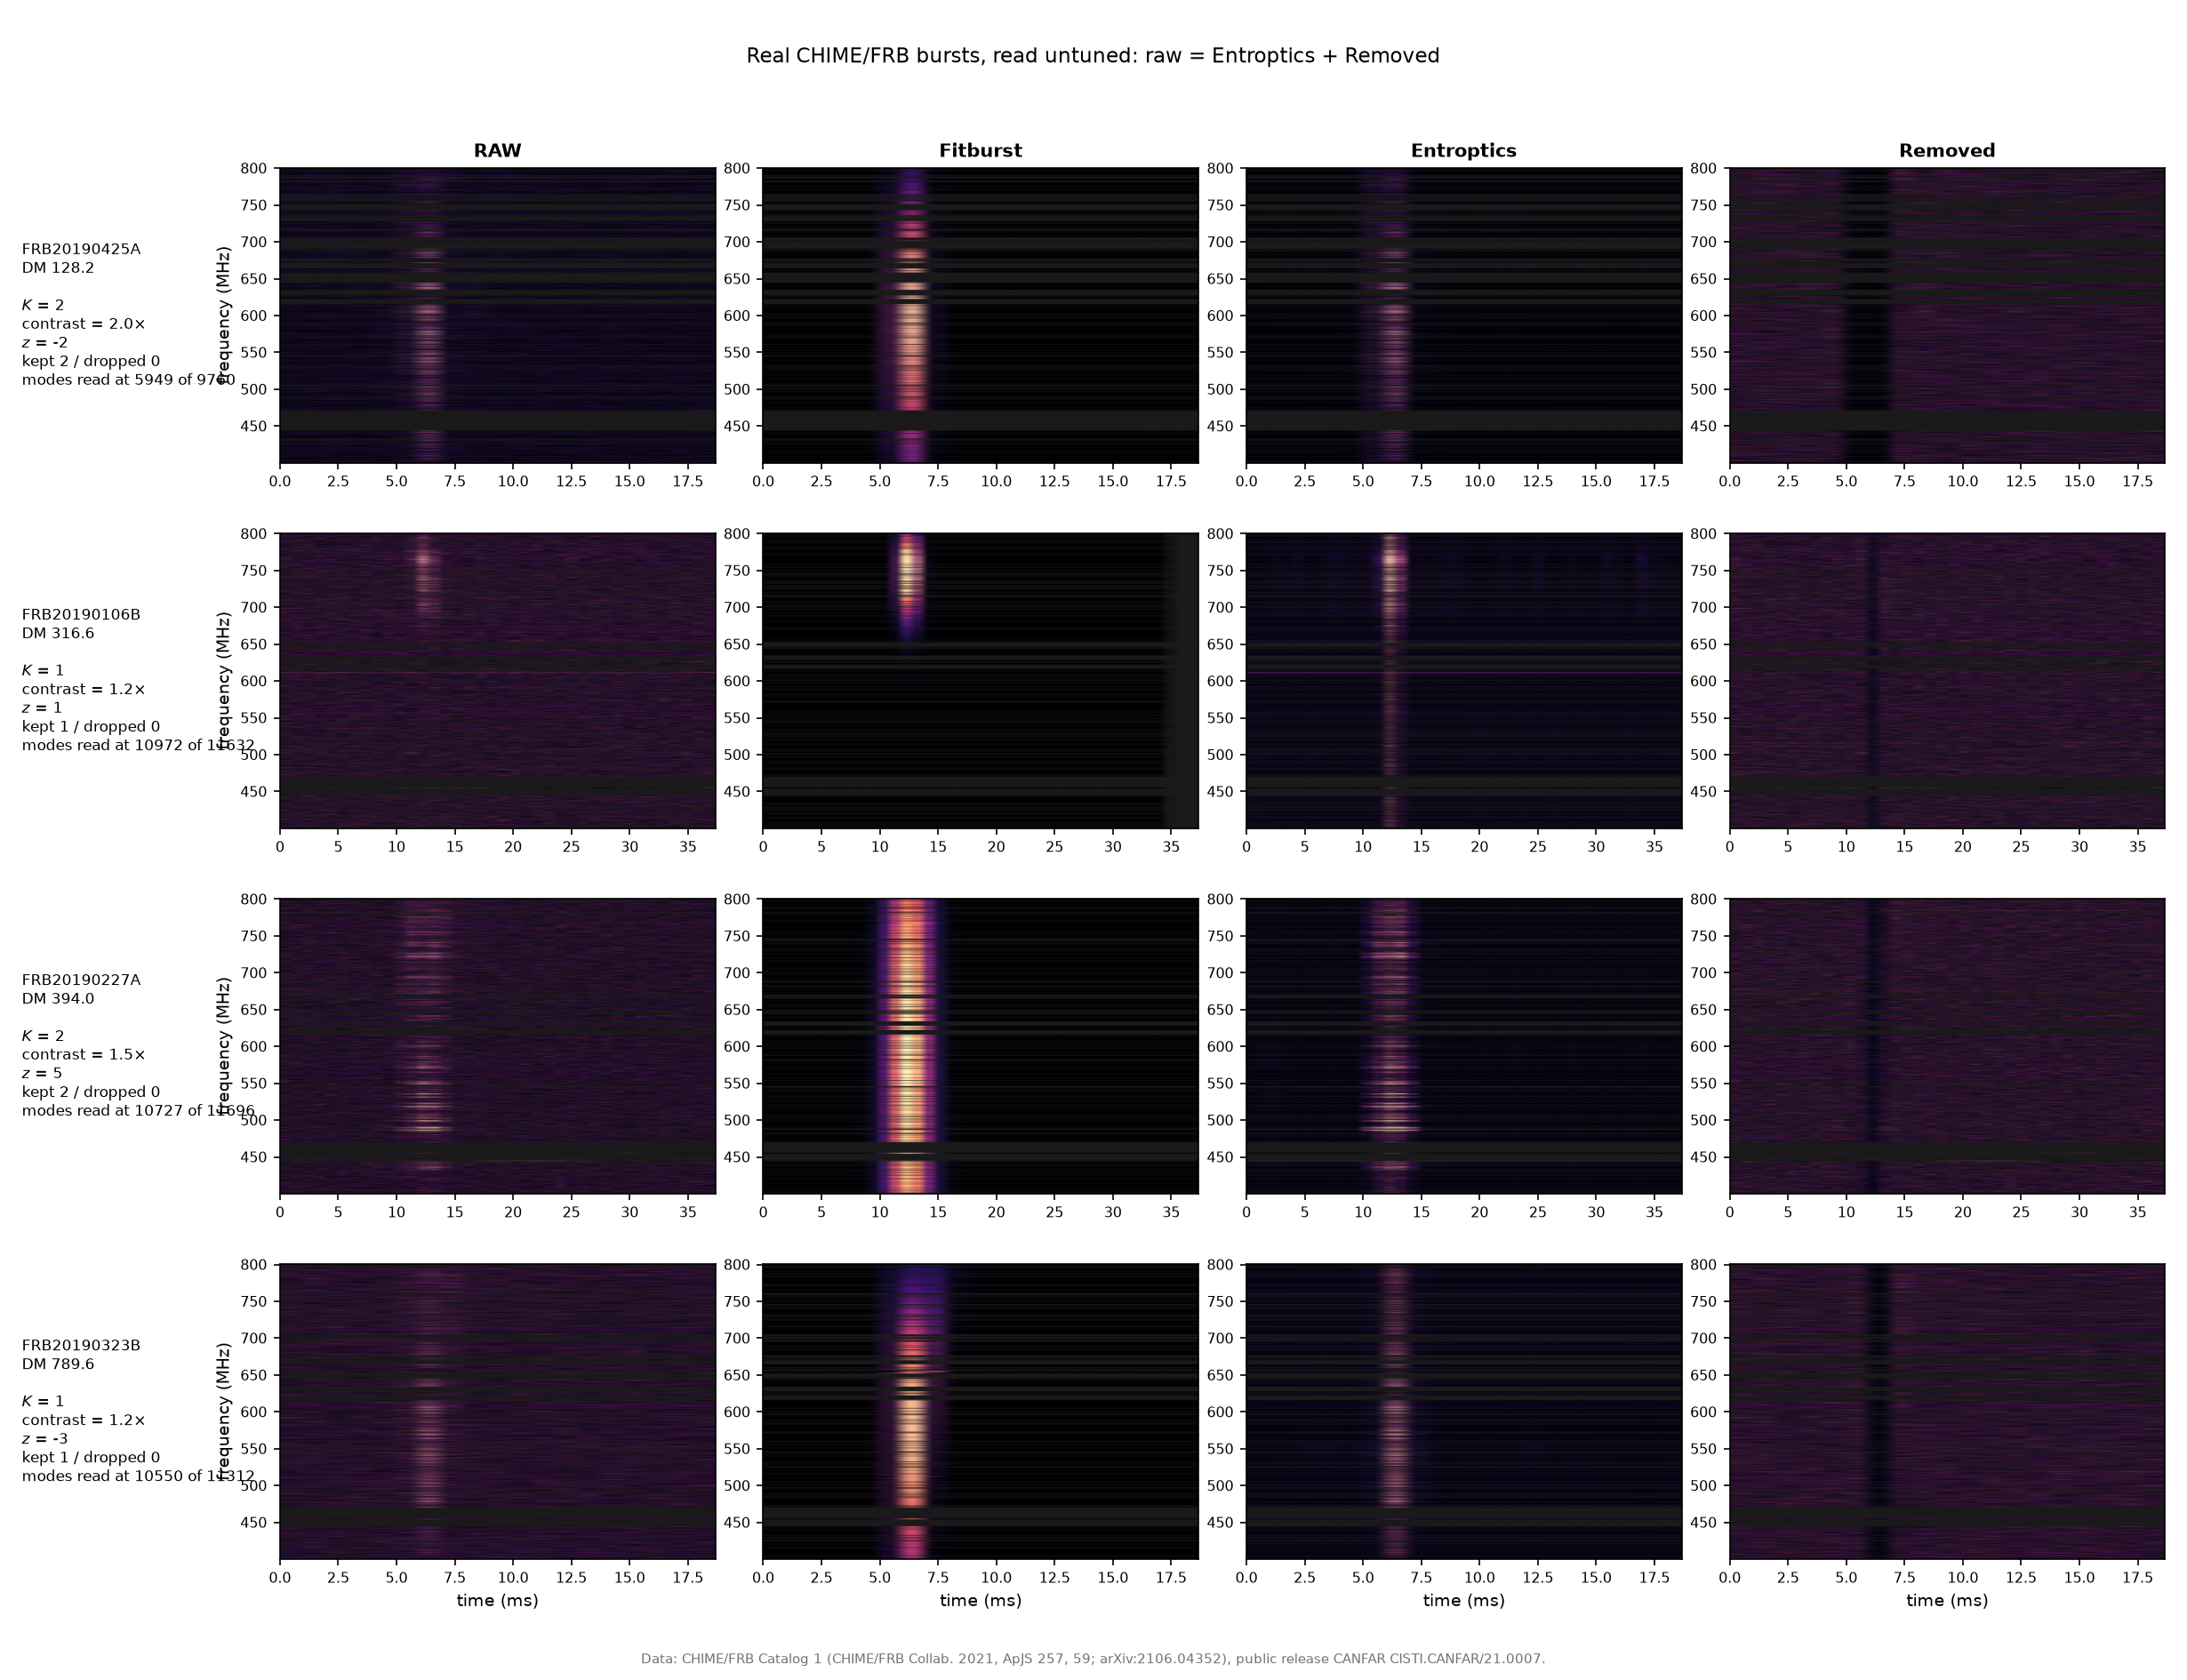
\includegraphics[width=\textwidth,height=0.8\textheight,keepaspectratio]{figures/frb_panel.png}
\caption*{Figure 1. Four CHIME/FRB Catalog 1 bursts read untuned, one row per
event. Left to right: the raw dedispersed waterfall, CHIME's
\emph{fitburst} forward model, the reconstruction, and what the read did
not keep. Each panel is contrast-stretched independently between its own
median and 99.7th percentile --- the four hold quantities on different
scales, and the model in particular is noiseless and non-negative --- so
the comparison to make by eye is of morphology and not of contrast.}
\end{figure*}

\begin{table*}[tp]
\centering\footnotesize
\caption*{\emph{Table 1. Per-burst reads, from
\texttt{tables/\allowbreak{}events.\allowbreak{}csv}. ``live'' is the
surviving width of the 16,384 recorded channels; ``read at'' is the
width the modes are read at, the fold's. Contrast is \(\sigma_1/\Phi\),
the leading singular value over the screen floor; \(z\) is the
ordered-axis coherence. ``kept'' and ``dropped'' are the resolved modes
on each side of the geometry cut.}}
\typesetfit{\textwidth}{%
\begin{tabular}{llllllllll}
\toprule
event & DM & \(T\) & live & read at & \(K_{\mathrm{signal}}\) & contrast & \(z\) & kept & dropped \\
\midrule
FRB20190425A & 128.2 & 19 & 9,760 & 5,949 & 2 & 2.03 & −2.5 & 2 & 0 \\
FRB20190106B & 316.6 & 38 & 11,632 & 10,972 & 1 & 1.17 & 1.3 & 1 & 0 \\
FRB20190227A & 394.0 & 38 & 11,696 & 10,727 & 2 & 1.48 & 5.2 & 2 & 0 \\
FRB20190323B & 789.6 & 19 & 11,312 & 10,550 & 1 & 1.22 & −3.5 & 1 & 0 \\
\bottomrule
\end{tabular}}
\end{table*}

Each event resolves at least one mode above the floor. The reported per-mode quantity is the bounded contrast \(\sigma_1/\Phi\).

The record shapes are extreme --- \(T=19\)--\(38\) against \(16{,}384\) recorded channels --- so the aspect ratio each read was taken at is on the page beside it.

The modes are read at the fold's width (the ``read at'' column), and every recorded channel is then projected onto them, so the read is at the recorded frequency resolution.

\subsection{3.2 A random spot-check}\label{32-a-random-spot-check}

A further 12 waterfalls, drawn uniformly at random from the same public release, at a fixed seed, are read by the identical path (\texttt{tables/\allowbreak{}spotcheck.\allowbreak{}csv}). All twelve are read without incident, and \(K_{\mathrm{signal}}\ge1\) on eight of them.

The four that resolve nothing are the four whose leading singular value sits at or below the derived floor --- contrast \(0.99\)--\(1.00\), against \(1.17\)--\(2.03\) for the events of Figure 1 --- the floor declining to certify a mode it cannot separate from the bulk. Record length does not separate the two groups: the four that resolve nothing span \(T=19\)--\(57\) and the eight that resolve span \(T=19\)--\(95\), so the shortest records sit in both.

This establishes that the untuned instrument runs on records it was not selected against, and reports what it finds on them. It is not a performance measurement: nothing here is scored against a reference.

\subsection{3.3 Agreement with the forward model}\label{33-agreement-with-the-forward-model}

\emph{fitburst} is fitted with the shape of a burst already in it and solves for that shape's parameters. The read is given no model of a burst at all and keeps whatever modes clear the floor. The two share no assumptions, so agreement between them on the same waterfall is evidence that the read is finding the burst rather than an artifact of its own construction.

Every quantity is scored on the same cells (the live channels --- the read is undefined on dead ones, and scoring each series wherever it happens to be finite scores them on different pixels) and with its per-channel baseline removed. The baseline removal is what makes the series comparable, and it is applied to all of them: \texttt{model\_\allowbreak{}wfall} carries no per-channel standing level at all --- its per-channel median is numerically zero, at most \(3.9\times10^{-6}\) across the four events against model maxima of \(0.108\)--\(0.506\) --- because it is a statement about the burst and not about each channel's baseline. A series carrying a baseline would therefore be scored against one that does not, and the baseline would count as disagreement. Centring one series and not the others would hand that one a comparison the references never got.

\typesetcolumntable{%
\begin{tabular}{lll}
\toprule
series & range & mean \\
\midrule
raw waterfall & \(0.115\)--\(0.373\) & \(0.198\) \\
box-average control & \(0.118\)--\(0.427\) & \(0.214\) \\
\textbf{the read} & \(\mathbf{0.421}\)--\(\mathbf{0.533}\) & \(\mathbf{0.470}\) \\
\bottomrule
\end{tabular}}

\emph{Table 2. Correlation against the fitburst forward model, from \texttt{tables/\allowbreak{}agreement.\allowbreak{}csv}.}

The model is smooth along frequency, so the box-average control rebins the raw waterfall to the width the modes are read at --- smoothing alone, with no read. It reads \(0.214\). Smoothing accounts for \(6.1\%\) of the gain and the read for the rest. The read itself is not smoothed: it is at the recorded channel resolution, and keeps structure along frequency that the smooth model does not carry.

\section{4. What sets the scale}\label{4-what-sets-the-scale}

A correlation of \(0.470\) against a series that is not ground truth means nothing on its own. There is no ground truth here to supply a scale --- the source of a fast radio burst is unknown, and the forward model is a parametric fit to the same waterfall --- so we report two reference points that are computable from the record itself and say what each does and does not bound.

\textbf{The noise-limited reference.} Take the forward model itself, corrupt it with this record's own per-channel noise, and score it against the model. The noise scale is read robustly (MAD) from the off-burst columns of the raw waterfall, where the on-burst window is the smallest contiguous run of time samples containing \(99\%\) of the model's band-summed power --- a stated criterion, and the only free choice in this section. This answers: \emph{what would a method that recovered the forward model exactly score, if it were measured through this waterfall's noise?}

\textbf{The fold-resolution ceiling.} Take the forward model, degrade it by exactly the fold the read is taken at, and score it against the model. This answers: \emph{what is the most a read limited to that frequency resolution could score, from resolution alone?} The read itself is taken back to the recorded channels and is not bound by it.

\typesetcolumntable{%
\begin{tabular}{L{0.621\linewidth}L{0.190\linewidth}L{0.086\linewidth}}
\toprule
reference & range & mean \\
\midrule
noise-limited (perfect recovery, measured through this noise) & \(0.117\)--\(0.439\) & \(0.219\) \\
raw waterfall (measured) & \(0.115\)--\(0.373\) & \(0.198\) \\
\textbf{the read} & \(\mathbf{0.421}\)--\(\mathbf{0.533}\) & \(\mathbf{0.470}\) \\
fold-resolution ceiling (perfect recovery at the read's resolution) & \(0.9853\)--\(0.9987\) & \(0.994\) \\
\bottomrule
\end{tabular}}

\emph{Table 3. The read against its two reference points, from \texttt{tables/\allowbreak{}agreement.\allowbreak{}csv}.}

Two things follow, and they are the point of the section.

\textbf{The raw waterfall's low agreement is noise, not disagreement about the burst.} A series that \emph{is} the forward model, measured through this record's noise, scores \(0.219\); the raw waterfall scores \(0.198\). The two are not meaningfully different. So the forward model's functional form is not what holds the raw frame down to \(0.198\) --- the noise is, entirely. That is the floor the read has to beat, and it beats it on every event.

\textbf{Resolution is not what caps the read.} A perfect recovery at the modes' folded width scores \(0.994\). The fold costs at most \(1.5\%\) of the attainable correlation on the worst of the four events and \(0.1\%\) on the best. So the gap between \(0.470\) and \(1\) is not the resolution the instrument chose.

\textbf{What we cannot bound.} The remaining gap is attributable to the forward model's own form. \emph{fitburst} is smooth and has no per-channel freedom, while both the waterfall and the read carry per-channel structure that no smooth parametric surface can represent. Quantifying that would require refitting \emph{fitburst} --- perturbing its parameters, or refitting it to a resampled record --- and we do not have its fitting code. We therefore do not report a ceiling that accounts for the model's form, and the residual gap between \(0.470\) and \(0.994\) should not be read as error in the read. It is a mixture of the read's own residual and a representational limit of the reference, in unknown proportion.

One consequence of scoring on the full frame is worth naming. Off the burst, both the read and the model are close to zero, and that agreement counts toward the score. Restricted to the on-burst window alone, the raw waterfall reads \(0.297\) and the read \(0.394\) (means; per-event values in \texttt{tables/\allowbreak{}agreement.\allowbreak{}csv}). The read's margin over the raw survives the restriction --- the read is \(2.4\times\) the raw on the full frame and \(1.3\times\) on the on-burst window --- but the absolute figures are lower, and a reader comparing against a full-frame number elsewhere should use the same convention.

\section{5. Limits}\label{5-limits}

\textbf{Neither is ground truth.} The source of a fast radio burst is unknown, and the forward model is itself a fit to this same waterfall with no per-channel freedom. The agreement says that two methods assuming nothing in common find the same burst; it does not say either has recovered it correctly.

\textbf{The floor's null is an i.i.d. bulk, and that is a real restriction.} The Tracy--Widom law the floor is derived from is the null of independent channels, each i.i.d. in time. Noise correlated \emph{across} channels --- common-mode drift, narrowband interference --- concentrates its variance into a few modes and is, on the singular spectrum alone, indistinguishable from signal; the floor counts it as resolved. The read is a correlation read, so a mode must span channels to clear the edge --- about \((1+\sqrt{F_{\mathrm{eff}}/T})^2\) of them --- and a structure confined to fewer, such as a single-channel line, is not resolved at any strength. Correlation \emph{along} the ordered axis moves the bulk itself. Measured on pure AR(1) rows with no planted signal, the derived floor resolves a mode in \(100\%\) of draws at every correlation length from \(\rho=2\) to \(32\), against \(0\)--\(2.5\%\) on i.i.d. rows {[}Sessford 2026, §12{]}. The effect is in the spectrum rather than in any estimator: at shape \((200,200)\) and \(\rho=2\) the leading singular value of the raw field averages \(37.5\) against a Bai--Yin i.i.d. edge of \(28.3\), with \(13.3\) values above it, where the i.i.d. control sits on the edge at \(28.0\) with \(0.1\). No method reading against that edge can be right on such a record, and the standard singular-value and model-order selectors over-read the same records by two to four times as much.

What this bounds is a record whose \emph{noise} is correlated along the ordered axis. A dedispersed waterfall, whose noise is close to white in time, is not affected, and the reads above are not. A record carrying \(1/f\) drift or a common-mode gain would be.

\textbf{The geometry cut is a criterion, not a test.} It carries no null and no level, and it drops persistent structure whether or not that structure is interference. A genuinely persistent narrowband astrophysical signal would be removed by it.

\textbf{The sample is small.} Four events with a figure and twelve more read blind is a demonstration of transfer, not a survey. Nothing here supports a population statement about Catalog 1.

\section{6. Reproduction}\label{6-reproduction}

Every number in this paper is written by one script:

\begin{verbatim}
python reproduce.py
\end{verbatim}

It runs the two committed figure routines (\texttt{figures/\allowbreak{}frb\_\allowbreak{}panel.\allowbreak{}py}, \texttt{figures/\allowbreak{}frb\_\allowbreak{}spotcheck.\allowbreak{}py}) and writes three tables beside itself:

\typesetcolumntable{%
\begin{tabular}{L{0.234\linewidth}L{0.429\linewidth}L{0.234\linewidth}}
\toprule
table & holds & used in \\
\midrule
\texttt{tables/\allowbreak{}events.\allowbreak{}csv} & per-burst reads for the four events & Table 1, §3.1 \\
\texttt{tables/\allowbreak{}spotcheck.\allowbreak{}csv} & the 12-waterfall random draw & §3.2 \\
\texttt{tables/\allowbreak{}agreement.\allowbreak{}csv} & every correlation, including both references & Tables 2 and 3, §§3.3, 4 \\
\bottomrule
\end{tabular}}

The script imports \texttt{entroptics} and calls its public front door; it reimplements nothing. Every seed is fixed and the tables are byte-reproducible across runs.

\textbf{The data is a separate download.} The CHIME/FRB Catalog 1 waterfalls are a public release from the CANFAR archive (CISTI.CANFAR/21.0007) and are not part of the software repository. \texttt{README.\allowbreak{}md} beside this paper documents the fetch and the one line of configuration that points the scripts at it. No script here downloads the release: it is far larger than a reproduction script should pull unasked, and a partial download would overwrite good tables with empty ones while still exiting zero. The scripts refuse, with instructions, if they find nothing.

\section{Declaration of generative AI use}\label{declaration-of-generative-ai-use}

The author used Anthropic's Claude Opus (versions 4.8, 5, and 5.5) in the preparation of this work. Its
contribution was to write code, and to generate and validate content. The ideas, the construction
and the claims are the author's. No other generative AI tool was used. The author reviewed and
edited all output and takes full responsibility for the content of this publication.

\section{References}\label{references}

\begin{itemize}
\tightlist
\item
  Z. Bao, G. Pan, W. Zhou, \emph{Tracy--Widom law for the extreme eigenvalues of sample correlation matrices}, Electron. J. Probab. \textbf{17} (2012) no. 88, 1--32.
\item
  CHIME/FRB Collaboration, \emph{The First CHIME/FRB Fast Radio Burst Catalog}, Astrophys. J. Suppl. Ser. \textbf{257} (2021) 59, arXiv:2106.04352. Data (public): CANFAR archive, CISTI.CANFAR/21.0007, \url{https://www.canfar.net/}.
\item
  I. M. Johnstone, \emph{On the distribution of the largest eigenvalue in principal components analysis}, Ann. Statist. \textbf{29} (2001) 295--327.
\item
  I. J. Sessford, \emph{Entroptics: reading a 2-D signal as a finite optical aperture at its own entropy-matched resolution}, pre-print, 2026. \href{https://github.com/Agience/entroptics}{https:\allowbreak{}/\allowbreak{}/\allowbreak{}github.\allowbreak{}com/\allowbreak{}Agience/\allowbreak{}entropti\allowbreak{}cs}
\item
  C. A. Tracy, H. Widom, \emph{On orthogonal and symplectic matrix ensembles}, Comm. Math. Phys. \textbf{177} (1996) 727--754.
\item
  Y. Q. Yin, Z. D. Bai, P. R. Krishnaiah, \emph{On the limit of the largest eigenvalue of the large dimensional sample covariance matrix}, Probab. Theory Related Fields \textbf{78} (1988) 509--521.
\item
  Z. D. Bai, Y. Q. Yin, \emph{Limit of the smallest eigenvalue of a large dimensional sample covariance matrix}, Ann. Probab. \textbf{21} (1993) 1275--1294.
\item
  E. B. Wilson, M. M. Hilferty, \emph{The distribution of chi-square}, Proc. Natl. Acad. Sci. USA \textbf{17} (1931) 684--688.
\end{itemize}

\end{document}
